\section{Improvements}
\subsection{Considerations about number of birds}
If we study the effects of how different number of birds change the solution of different tours, we learn that less birds seem to yield better solutions. At first this may seem counterintuitive, but there is an intuitive explanation to this:

The basic algorithm defines one iteration as the calculation for the cost of one tour. Now, let a phase of the algorithm denote each bird performing one move. So, in each phase each bird performs one move.
If we now use more birds the number of phases the algorithm will run through will decrease, as in each phase the length of more tours will be calculated, which will use up more iterations. Therefore, the more birds we have, the more iterations we will use up per phase, which means the algorithm will run through less phases until it stops. 
Because in one phase each bird can perform one move, less phases mean each bird can perform less moves. Less moves in turn leads to a less pronounced search of possible solutions, which will make the algorithm worse. This is why the less birds we have, the better the results will be.

Consequently, we aim to improve the bird behaviour, so that each bird needs fewer overall steps to achieve a good solution.

\subsection{Swarm behaviour}
Currently, if one big bird made the decision to join another bird, he picks one randomly.
This means joining any bird without considering how good the position of that bird might be. This contradicts the original idea of the authors that big birds tend to join others that have found a good food source (current solution seems promising).
Therefore, we propose that a big will only be able to join the top-b percent of birds that have the lowest current cost. If one chooses the right ratio, we assume that it will automatically nudge the swarm in the direction of the global minimum.

We implement this by storing the indices $i$ of the birds in an ordered integer array $ord$ and introducing a new hyperparameter call $b$, denoting which of the top-b percent to join. When we select the bird to join to, we draw a random uniform number $j$ between 1 and $b*n$ ($n$ denotes the number of birds) and get the index of the bird to join from the ordered array ($ord[j]$).

The main disadvantage this approach has is that at we need to continuously update $ord$ so that we only join the actual top-b percent at the moment of the move. We decide to update the list after each bird has performed one move, so after each phase.

We test numerous values for $b$ and decide to build on $b=0.01$ for future improvement, as this strategy yields the best results. For intuitions on why such a low value performs this good, please refer to section "NOCH HINZUFÜGEN".

\subsection{3-opt Walk}

For the walk move the Algorithm uses a modified version of the 2-opt heuristic as a local search. Instead of using 2-opt, we test a 3-opt variant, as this often yields the best solutions under consideration of computational complexity \cite{lin}. At the same time we decide to remove the estimation of local similarity from the algorithm, as the authors did not provide any intuitions why this may be beneficial \cite{afb}.

With this variant, each bird selects the tour with the lowest cost out of the 7 different tours possible in 3-opt. At which 3 points a tour is opened is determined by a random uniform draw of 3 integers, denoting the indices of the tour. Because we need to calculate the length of each of the possible 7 tours, and this happens in just one move of one bird, this move still only costs one iteration.

\begin{figure}[htbp]
\centerline{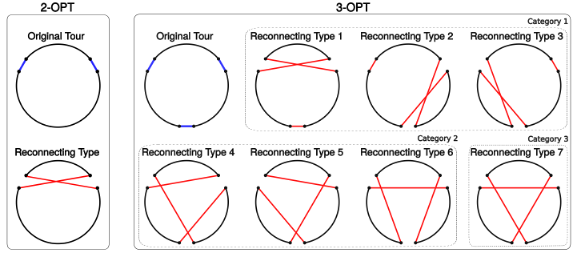
\includegraphics[width=8cm]{3_opt}}
\caption{\cite{3_opt}}
\label{3_opt}
\end{figure}

The results can be seen in ... .

\subsection{Delegating Responsibility}

Because we are not implementing the 3-opt algorithms by itself, but rather in a swarm algorithm, in which each bird (or agent respectively) can perform this action, the computational complexity will rise by a margin, as seen in Table <…>. This is why we test the case where only big birds are able to perform a 3-opt walk, while smaller birds are only capable of the usual 2-opt walk as specified in the paper. This should not only reduce the computational complexity but also pairs well with the assumption that big birds are superior, as only they can join other birds and therefore profit from them.

Furthermore, we also test the inverse approach: Only small birds can perform 3-opt.
Based on the results we decide to use 3-opt for big birds from, as this provides the best average improvement in performance with a reasonable increase in computation time.

\subsection{Nearest-Neighbor Initialization}

\subsection{Intuitions on Improvements}